\section{Overview of the Simulation Tool PROPOSAL}\label{sec:proposal}
The tool PROPOSAL propagates charged leptons and photons through media und is 
used in this paper to simulate the deflection of muons. For this purpose, 
negative charged muons $\mu^-$ are propagated through the media ice and water 
\alexander{Wofür ist es wichtig, daß die Myonen negativ geladen sind?
Sind nicht alle Wirkungsquerschnitte und Ablenkungsparametrisierungen davon
unabhängig?}
to estimate the deflection for IceCube and KM3NeT/ARCA. All relevant muon interaction types 
as bremsstrahlung \cite{KKP_1995, Karnaukhov_1999}, photonuclear interaction \cite{Abramowicz_1997} with 
shadowing \cite{ButkevichMikheyev_2002}, electron pair production \cite{KKP_proc} with corrections for the 
interaction with atomic electrons \cite{Kelner_1998}, 
ionization by Bethe-Bloch formula with corrections for muons \cite{Rossi} and decay are provided. The interaction processes are sampled by their cross section. Since bremsstrahlung interactions can be 
arbitrary small due to a massless exchange particle, the photon, an energy cut is introduced to avoid an infinite number of bremsstrahlung interactions 
and furthermore to speed up the propagation process. 
The limit is applied with a minimum energy loss
\begin{equation}
    E_{\text{loss,min}} = \min{(E \cdot \texttt{v\_cut}, \texttt{e\_cut})}\,,
\end{equation}
using two parameters - a relative and total energy cut denoted as 
$\texttt{v\_cut}$ and $\texttt{e\_cut}$ with particle energy $E$. The uncertainties are small 
for a relative energy cut $\texttt{v\_cut}\ll 1$, which increases the 
CPU runtime.
A sampled energy loss 
$E_{\text{loss}} < E_{\text{loss,\,min}}$ builds an integrated part of a 
stochastic energy loss referred to as continuous energy loss. The 
propagation process is defined by an initial energy $E_{\text{i}}$ and 
two stopping criteria - a final energy $E_{\text{f,\,min}}$ and a 
maximum propagation distance $d_{\text{min}}$. If the last interaction of 
a propagation is sampled by a stochastic interaction, the true final energy 
$E_{\text{f}}$ can become lower and the 
propagation distance $d$ can be higher than the required limits. 
The deflections for stochastic interactions are parametrized by Van Ginneken 
in \cite{Van_Ginneken} with a direct calculation of the deflection in 
ionization using four-momentum conservation. 
Furthermore, there are parametrizations for deflections given in GEANT4 \cite{GEANT4} 
for bremsstrahlung and photonuclear interaction, which 
are available in PROPOSAL, too.
To estimate the deflection along 
a continuous energy loss, multiple scattering established by Moliére 
\cite{moliere_scattering} and the gaussian approximation by Highland 
can be chosen \cite{HIGHLAND_1975}. 
The deflection angle in the plane perpendicular to the muon direction is 
sampled uniformly between $0$ and $2\pi$.
The latest updates with a detailed description of the whole tool can be found 
in \cite{phd_soedingrekso}.
All simulations are done with PROPOSAL $7.3.0$.

\section{Muon deflection per Interaction}\label{sec:defl_per_int}
First, the stochastic deflections introduced by \cite{Van_Ginneken} implemented 
in PROPOSAL are investigated in relation to the two multiple scattering methods. Thereby, the deflections per interaction are presented 
for each interaction type and the total amount in Figure~\ref{fig:defl_per_int}. A single deflection 
extend over several orders of magnitude with a median of $\SI{3.9e-6}{\degree}$
and a $\SI{95}{\percent}$ central interval of $[\SI{4.9e-7}{\degree}, \,\SI{1.3e-3}{\degree}]$. 
\alexander{Die Energien sollten nicht nur in der Bildunterschrift stehen.}
It follows that the deflections are primarily dominated by multiple scattering, except for a few outliers caused by bremsstrahlung, which 
allows very large energy losses and thus the largest deflections.
The median propagation distance with the lower and upper $\SI{95}{\percent}$ 
interval results to $16.4_{-7.3}^{+24.6}\,\si{\kilo\meter}$.

\begin{figure}
    \centering 
    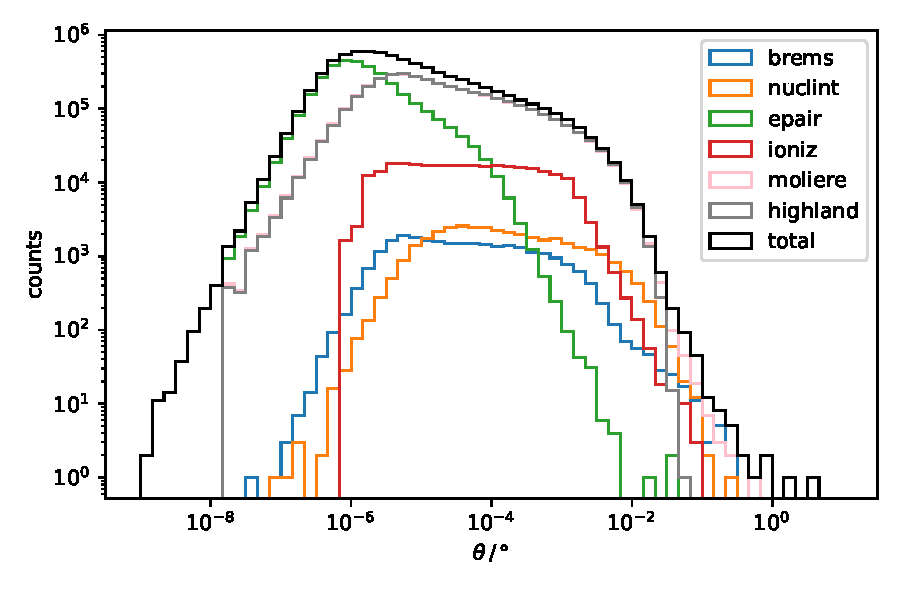
\includegraphics[width=0.8\textwidth]{figures/1PeV_1TeV_1000events_moliere_ecut500_vcut0.05_interpol200_vG_binning_paper.pdf}
    \caption{The deflection $\theta$ per interaction is shown in degree for different mechanisms. The propagation is done for $\num{1000}$ 
    muons from $E_{\text{i}} = \SI{1}{\peta\electronvolt}$ to $E_{\text{f,\,min}} = \SI{1}{\tera\electronvolt}$ using $\texttt{e\_cut} = \SI{500}{\mega\electronvolt}$ and $\texttt{v\_cut} = 0.05$ in ice. Two simulations 
    are done to check both multiple scattering methods Molière and Highland. The total distribution includes all stochastic processes and Molière's. Multiple scattering dominates the deflection. Details are presented in 
    Table~\ref{tab:defl_per_int}.}
    \label{fig:defl_per_int}
\end{figure}

\begin{table}
    \centering 
    \caption{The medians of deflections $\theta$ per interaction from Figure~\ref{fig:defl_per_int} are presented for each interaction type and the total distribution with the upper and lower limits of the $\SI{95}{\percent}$ 
    central content levels.}
    \begin{tabular}{ccccccc}
        \toprule 
        brems & nuclint & epair & ioniz & moliere & highland & total \\
        $\theta\,/\,\SI{e-5}{\degree}$ & $\theta\,/\,\SI{e-4}{\degree}$ & $\theta\,/\,\SI{e-6}{\degree}$ & $\theta\,/\,\SI{e-5}{\degree}$ & $\theta\,/\,\SI{e-5}{\degree}$ & $\theta\,/\,\SI{e-5}{\degree}$ & $\theta\,/\,\SI{e-6}{\degree}$\\
        \midrule 
        $3.8_{-0.1}^{+297}$ & $1.2_{-0.4}^{+96}$ & $1.3_{-0.2}^{+42}$ & $4.4_{-0.1}^{+181}$& $1.2_{-0.05}^{+222}$ & $1.2_{-0.05}^{+225}$ & $3.9_{-0.2}^{+1285}$\\ 
        \bottomrule
    \end{tabular}
    \label{tab:defl_per_int}
\end{table}
